\documentclass{article}
\usepackage{amsmath}
\usepackage{amssymb}
\usepackage{graphicx}
\usepackage{enumitem}
\usepackage[utf8]{inputenc}
\graphicspath{{/home/stephanie/Escritorio/THC/Taller-de-Herramientas-Computacionales/Clases/Latex/Imagenes/}}

\title{\Huge Taller de Herramientas Computacionales}
\author{Stephanie Escobar Sánchez}
\date{22/enero/2019}

\begin{document}
	\maketitle
	\begin{center}
		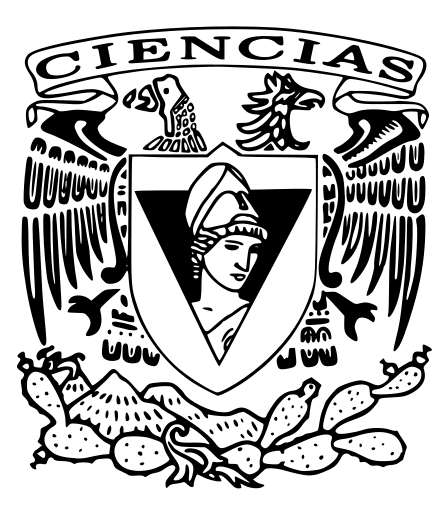
\includegraphics[scale=0.40]{1.png}	
	\end{center}
	\newpage
	\title{\Huge Bitácora clase 12} \\
	\\
	
	input(archivo)
	include (archivo)
	range(len) para recorrer por los indices 
	Sublistas es algo interesante que tienen los lenguajes, A [2:] es regresa a partir del índice 2 
	A[1:3] del uno hasta antes del 3 
	A[1:-1] todos los anteriores al índice que puse
	A[1:-1] regresa todos exepto el primero y el último 
	Las distas de python son de alguna forma listas circulares como si el último elemento estuviera conectado con el primero 
	Tabla[4:7][0:2] Nos regresa una lista dentro de la lista
	Cuando gusrdamos las variables son dos objetos independientes 
	: son para obte 
	ner sublistas B=A[:] es una sublista que contiene una copia de los elementos de A
	¿Cuando dos listas son iguales?
	si contienen los mismos elementos y se usa ==
	Si yo quiero saber si es el mismo objeto le pregunto con is,
	c = a los hace iguales, si modifico cualquiera de las 2 pues cambia 
	Cuando hablamos de un objeto hay atributos y métodos y estan guardadas en una memoria.
	Las variables también se convierten en identificadores de una sección de memoria, cual? una que contiene algo muy específico. Nos sirve igualarla para cuando es más evidente a la hora de escribir las variables.  Sirve para eviitar un error cuando es una copia. Utilizar python con referencias a las listas nos permite un códico más dinámico.
	si quiero recorrer una lista por indices:
	for i in rage
	si es por sus valores es el nombre de la lista
	
	paquetes en latex con vimer para presentación
	
presentaciones en latex
	
\end{document}